% !TeX program = xelatex
\documentclass[aspectratio=169,11pt]{beamer}

% -------------------------------------------------
% Packages
% -------------------------------------------------
\usepackage{kotex}
\usepackage{fontspec}
\usepackage{amsmath,amssymb,bm,mathtools}
\usepackage{booktabs,array}
\usepackage{xcolor}
\usepackage{colortbl}
\usepackage{tikz}
\usetikzlibrary{positioning,arrows.meta,calc,fit,decorations.pathreplacing}
\usepackage[most]{tcolorbox}
\usepackage{listings}
\usepackage{adjustbox}

% -------------------------------------------------
% Colors (same as the notes)
% -------------------------------------------------
\definecolor{deepblue}{RGB}{34,71,120}
\definecolor{softblue}{RGB}{239,246,253}
\definecolor{softgray}{RGB}{246,247,249}
\definecolor{softgreen}{RGB}{239,249,242}
\definecolor{softyellow}{RGB}{255,249,229}
\definecolor{codegray}{RGB}{248,248,248}

% -------------------------------------------------
% Beamer look
% -------------------------------------------------
\usetheme{default}
\usefonttheme[onlymath]{serif}
\setbeamertemplate{navigation symbols}{}
\setbeamersize{text margin left=8mm,text margin right=8mm}
\setbeamercolor{structure}{fg=deepblue}
\setbeamercolor{frametitle}{fg=deepblue}
\setbeamercolor{title}{fg=deepblue}
\setbeamerfont{frametitle}{size=\large,series=\bfseries}
\setbeamertemplate{itemize items}[circle]
\setbeamertemplate{enumerate items}[default]
\setbeamertemplate{frametitle}{%
  \vskip3mm
  {\usebeamerfont{frametitle}\usebeamercolor[fg]{frametitle}\insertframetitle\par}%
  \vskip1mm
  {\color{deepblue!45}\hrule height 0.6pt}%
  \vskip1mm}
\setbeamertemplate{footline}{%
  \hbox to\paperwidth{%
    \hspace*{8mm}{\color{black!45}\scriptsize CNN: PyTorch 코드 읽기\ifx\insertsectionhead\empty\else\ \ $\cdot$\ \ \insertsectionhead\fi}%
    \hfill{\color{black!45}\scriptsize\insertframenumber\,/\,\inserttotalframenumber}\hspace*{8mm}}%
  \vskip2.5mm}
\setbeamertemplate{title page}{%
  \vfill
  \begin{center}
  {\color{deepblue}\Huge\bfseries\inserttitle\par}
  \vskip3mm
  {\color{deepblue!60}\rule{9cm}{0.8pt}\par}
  \vskip3mm
  {\large\insertsubtitle\par}
  \vskip8mm
  {\normalsize\insertdate\par}
  \end{center}
  \vfill}
\AtBeginSection[]{%
  \begin{frame}
  \vfill
  \centering
  {\color{deepblue!55}\Large\bfseries \insertsectionnumber\par}
  \vskip2mm
  {\color{deepblue}\LARGE\bfseries\insertsectionhead\par}
  \vskip3mm
  {\color{deepblue!50}\rule{7cm}{0.8pt}\par}
  \vfill
  \end{frame}}
\setlength{\leftmargini}{1.2em}
\addtobeamertemplate{itemize/enumerate body begin}{}{\setlength{\itemsep}{0.2ex}}
\setlength{\leftmarginii}{1.1em}

% -------------------------------------------------
% Boxes (same colors as the notes)
% -------------------------------------------------
\newtcolorbox{keybox}[1][]{colback=softblue,colframe=deepblue,boxrule=0.7pt,arc=2mm,
  title=#1,fonttitle=\bfseries\small,left=2mm,right=2mm,top=1mm,bottom=1mm,
  toptitle=0.5mm,bottomtitle=0.5mm}
\newtcolorbox{thinkbox}[1][]{colback=softyellow,colframe=orange!70!black,boxrule=0.6pt,arc=2mm,
  title=#1,fonttitle=\bfseries\small,left=2mm,right=2mm,top=1mm,bottom=1mm,
  toptitle=0.5mm,bottomtitle=0.5mm}
\newtcolorbox{remarkbox}[1][]{colback=softgray,colframe=black!45,boxrule=0.5pt,arc=2mm,
  title=#1,fonttitle=\bfseries\small,left=2mm,right=2mm,top=1mm,bottom=1mm,
  toptitle=0.5mm,bottomtitle=0.5mm}

% -------------------------------------------------
% Code style
% -------------------------------------------------
\lstdefinestyle{pythonstyle}{
  language=Python,
  backgroundcolor=\color{codegray},
  basicstyle=\ttfamily\fontsize{7.6}{8.6}\selectfont,
  keywordstyle=\bfseries\color{deepblue},
  commentstyle=\itshape\color{black!55},
  stringstyle=\color{black!75},
  numbers=none,
  frame=single,
  rulecolor=\color{black!25},
  breaklines=true,
  showstringspaces=false,
  tabsize=4,
  columns=fullflexible,
  keepspaces=true,
  aboveskip=1mm,
  belowskip=1mm
}
\lstset{style=pythonstyle}
% program output: no Python colors, light green background
\lstdefinestyle{outstyle}{style=pythonstyle,language={},backgroundcolor=\color{softgreen}}
% smaller code for long listings
\newcommand{\codesmall}{\ttfamily\fontsize{7.4}{8.3}\selectfont}
\newcommand{\codetiny}{\ttfamily\fontsize{6.8}{7.6}\selectfont}

% -------------------------------------------------
% Math commands (same as the notes)
% -------------------------------------------------
\newcommand{\R}{\mathbb{R}}
\newcommand{\vect}[1]{\bm{#1}}
\newcommand{\T}{^{\mathsf T}}
\newcommand{\pd}[2]{\frac{\partial #1}{\partial #2}}

\newcommand{\figcap}[1]{\par\vskip1mm{\centering\footnotesize\color{black!70}#1\par}}
\newcommand{\code}[1]{\texttt{#1}}

\graphicspath{{slides_figures/}}

\title{CNN: PyTorch 코드 읽기}
\subtitle{\texttt{nn.Conv2d} $\cdot$ \texttt{nn.MaxPool2d} $\cdot$ \texttt{nn.Flatten} $\cdot$ \texttt{mnist\_cnn\_torch.py}}
\date{딥러닝개론및연습 $\cdot$ 2026년 2학기}

\begin{document}

% =================================================
\begin{frame}[plain]
\titlepage
\end{frame}

% =================================================
\begin{frame}{이번 시간의 핵심 질문}
\begin{keybox}[이번 시간의 핵심 질문]
\begin{itemize}
\item 합성곱 계층과 풀링 계층을 PyTorch로는 어떻게 쓸까?
\item 이미지를 $784$개로 펼치지 않고 넣으려면 텐서의 모양을 어떻게 해야 할까?
\item 완전연결 신경망의 PyTorch 코드에서 \textbf{무엇만 바꾸면} CNN이 될까?
\item 같은 코드를 GPU에서 돌리면 얼마나 빨라질까? 결과는 똑같을까?
\end{itemize}
\end{keybox}
\vskip2mm
\begin{center}
\large $\Rightarrow$ \textbf{\code{mnist\_cnn\_torch.py}를 처음부터 끝까지 읽는다}
\end{center}
\end{frame}

\begin{frame}{이번 시간부터는 PyTorch 코드로}
\begin{itemize}
\item 지금까지는 계층의 \code{forward}와 \code{backward}를 NumPy로 \textbf{직접} 만들었다
\begin{itemize}
\item 원리를 이해하기 위해서였다. 합성곱 계층도 노트에서 \code{im2col}로 직접 구현했다
\end{itemize}
\item 이제부터는 \textbf{PyTorch 코드}를 중심으로 읽는다
\begin{itemize}
\item 계층이 많아지고 데이터가 커질수록 직접 짠 코드는 느리고, 틀리기 쉽다
\item 연구와 산업에서 쓰는 코드는 대부분 PyTorch로 되어 있다
\item 같은 코드가 GPU에서 그대로 돈다
\end{itemize}
\item 그래도 우리는 각 줄 뒤에서 \textbf{무엇이 계산되는지} 알고 있다: 합성곱, 풀링, 역전파, Adam
\end{itemize}
\vskip1mm
\begin{keybox}
\small 이번 시간의 코드: \code{CNN/code/mnist\_cnn\_torch.py} (90줄), 작은 예제 모음 \code{cnn\_torch\_demo.py}
\end{keybox}
\end{frame}

\begin{frame}{학습목표}
\begin{enumerate}
\item 이미지 미니배치를 $(N, C, H, W)$ 모양의 텐서로 만들 수 있다
\item \code{nn.Conv2d}의 인자, 가중치의 모양, 출력 크기를 설명할 수 있다
\item \code{nn.MaxPool2d}와 \code{nn.Flatten}이 하는 일을 설명할 수 있다
\item 모델의 각 계층을 지날 때 텐서의 모양과 매개변수 수를 계산할 수 있다
\item 완전연결 신경망 코드와 CNN 코드의 \textbf{같은 점과 다른 점}을 설명할 수 있다
\item 학습한 첫 번째 합성곱 계층의 필터를 꺼내 그릴 수 있다
\end{enumerate}
\end{frame}

\begin{frame}{목차}
\small
\tableofcontents
\end{frame}

% =================================================
\section{완전연결 신경망 코드에서 무엇이 바뀌나}
% =================================================

\begin{frame}[shrink]{바뀌는 것은 세 곳뿐}
\centering
\small
\renewcommand{\arraystretch}{1.25}
\begin{tabular}{>{\raggedright}p{2.6cm}>{\raggedright}p{4.9cm}>{\raggedright\arraybackslash}p{5.0cm}}
\toprule
& \textbf{완전연결 (\code{mnist\_torch.py})} & \textbf{CNN (\code{mnist\_cnn\_torch.py})} \\
\midrule
입력의 모양 & \code{(N, 784)}: 한 줄로 펼침 & \code{(N, 1, 28, 28)}: \textbf{이미지 모양 그대로} \\
모델 & \code{Linear}, \code{ReLU}, \ldots & \code{Conv2d}, \code{MaxPool2d}, \code{Flatten} + \code{Linear} \\
최적화 기법 & SGD 또는 AdamW & Adam \\
\midrule
데이터 분할 & \multicolumn{2}{c}{\code{mnist\_data.py}: 훈련 55000 / 검증 5000 / test 10000 (같음)} \\
손실 함수 & \multicolumn{2}{c}{\code{nn.CrossEntropyLoss} (같음)} \\
학습 루프 & \multicolumn{2}{c}{순전파 $\to$ 손실 $\to$ \code{zero\_grad} $\to$ \code{backward} $\to$ \code{step} (같음)} \\
평가 & \multicolumn{2}{c}{\code{@torch.no\_grad()}, \code{model.eval()}, \code{argmax} (같음)} \\
\bottomrule
\end{tabular}
\vskip3mm
\raggedright
\begin{itemize}
\item PyTorch 입문에서 말한 그대로: \textbf{모델이 바뀌어도 학습 루프는 한 글자도 바뀌지 않는다}
\item 그래서 이번 시간의 중심은 \textbf{입력의 모양}과 \textbf{세 가지 새 계층}이다
\end{itemize}
\end{frame}

\begin{frame}{신경망의 구조: SimpleConvNet}
\centering
\begin{adjustbox}{max width=\linewidth}
\begin{tikzpicture}[>=Latex,
  lay/.style={draw,rounded corners=2pt,minimum width=14mm,minimum height=13mm,font=\small,align=center,inner sep=1pt},
  cv/.style={lay,fill=orange!25,draw=orange!80!black,very thick},
  pl/.style={lay,fill=blue!12,draw=blue!60!black,very thick},
  sh/.style={font=\scriptsize,align=center,text=black!70},
  node distance=6mm]
\node[font=\small,align=center] (in) {$X$};
\node[cv,right=4mm of in] (c1) {Conv2d\\{\scriptsize $5\times5$, 30개}};
\node[lay,right=of c1] (r1) {ReLU};
\node[pl,right=of r1] (p1) {MaxPool\\{\scriptsize $2\times2$}};
\node[lay,right=of p1] (f1) {Flatten};
\node[lay,right=of f1] (a1) {Linear};
\node[lay,right=of a1] (r2) {ReLU};
\node[lay,right=of r2] (a2) {Linear};
\draw[->] (in) -- (c1);
\draw[->] (c1) -- node[sh,below=6mm] {$(30,24,24)$} (r1);
\draw[->] (r1) -- (p1);
\draw[->] (p1) -- node[sh,below=6mm] {$(30,12,12)$} (f1);
\draw[->] (f1) -- node[sh,below=6mm] {$4320$} (a1);
\draw[->] (a1) -- node[sh,below=6mm] {$100$} (r2);
\draw[->] (r2) -- (a2);
\draw[->] (a2) -- ++(9mm,0) node[right,font=\small] {$10$};
\node[sh,below=6mm] at (in.south) {$(1,28,28)$};
\end{tikzpicture}
\end{adjustbox}
\figcap{데이터 하나의 모양 (미니배치 차원 $N$은 생략)}
\vskip2mm
\raggedright
\begin{itemize}
\item 노트에서 NumPy로 만든 \code{SimpleConvNet}과 \textbf{같은 구조}
\item 합성곱 $\to$ 풀링으로 이미지의 \textbf{특징}을 뽑고, 펼친 뒤 완전연결 계층 두 개로 분류한다
\item 마지막 \code{Linear}의 출력 $10$개가 점수(logits). softmax는 손실 함수 안에서 계산된다
\end{itemize}
\end{frame}

% =================================================
\section{데이터: $(N, C, H, W)$ 텐서}
% =================================================

\begin{frame}[shrink,fragile]{준비와 데이터 불러오기}
\begin{lstlisting}
import os
import time
import numpy as np
import matplotlib.pyplot as plt
import torch
from torch import nn
from torch.utils.data import TensorDataset, DataLoader

from mnist_data import load_mnist_split

FIG_DIR = os.path.join(os.path.dirname(os.path.abspath(__file__)), "..", "figures")
os.makedirs(FIG_DIR, exist_ok=True)

torch.manual_seed(0)
device = "cuda" if torch.cuda.is_available() else "cpu"
print(f"device: {device}")

x_train, t_train, x_val, t_val, x_test, t_test = load_mnist_split()   # 55000 / 5000 / 10000
\end{lstlisting}
\small
\begin{itemize}
\item 지난번 \code{mnist\_torch.py}와 \textbf{같다}. \code{time}은 epoch마다 걸린 시간을 재려고
\item \code{mnist\_data.py}는 같은 폴더에 복사해 둔 학습 관련 기술 주차의 모듈. 넘파이 배열 \code{(N, 784)}와 one-hot 정답을 준다
\end{itemize}
\end{frame}

\begin{frame}[shrink,fragile]{이미지 모양으로 되돌리기: \code{(N, 784)} $\to$ \code{(N, 1, 28, 28)}}
\begin{lstlisting}
def to_dataset(x, t):
    """images (N, 784) -> (N, 1, 28, 28) tensors, one-hot labels -> class indices"""
    return TensorDataset(torch.tensor(x, dtype=torch.float32).reshape(-1, 1, 28, 28),
                         torch.tensor(np.argmax(t, axis=1)))
\end{lstlisting}
\begin{columns}[T,onlytextwidth]
\begin{column}{0.52\textwidth}
\begin{lstlisting}
x = torch.arange(2 * 784, dtype=torch.float32).reshape(2, 784)
print(tuple(x.shape), "->", tuple(x.reshape(-1, 1, 28, 28).shape))
\end{lstlisting}
\begin{lstlisting}[style=outstyle]
(2, 784) -> (2, 1, 28, 28)
\end{lstlisting}
\end{column}
\begin{column}{0.44\textwidth}
\centering
\small
\renewcommand{\arraystretch}{1.15}
\begin{tabular}{cl}
\toprule
\textbf{차원} & \textbf{뜻} \\
\midrule
$N$ & 데이터(이미지) 수 \\
$C$ & 채널 수 (흑백 $1$, 컬러 $3$) \\
$H$ & 높이 ($28$) \\
$W$ & 너비 ($28$) \\
\bottomrule
\end{tabular}
\end{column}
\end{columns}
\vskip1mm
\small
\begin{itemize}
\item PyTorch의 합성곱 계층은 \textbf{4차원} 텐서 $(N,C,H,W)$를 받는다. 노트의 NumPy 구현과 같은 순서
\item \code{reshape(-1, 1, 28, 28)}: \code{-1}은 ``나머지에서 계산''. 784개를 다시 $28\times28$로 접는다 (펼쳤던 순서 그대로)
\item 정답은 지난번처럼 \code{argmax}로 클래스 번호 \code{(N,)}로
\end{itemize}
\end{frame}

\begin{frame}[fragile]{\code{DataLoader}}
\begin{lstlisting}
train_loader = DataLoader(to_dataset(x_train, t_train), batch_size=100, shuffle=True)
val_loader = DataLoader(to_dataset(x_val, t_val), batch_size=1000)
test_loader = DataLoader(to_dataset(x_test, t_test), batch_size=1000)
\end{lstlisting}
\begin{itemize}
\item 지난번과 같다. 다만 꺼내는 미니배치의 모양이 다르다:
\begin{itemize}
\item \code{xb}: \code{(100, 1, 28, 28)}, \ \code{yb}: \code{(100,)}
\end{itemize}
\item 훈련: $55000/100=550$개의 미니배치, 섞어서. 검증과 test: 1000개씩, 섞지 않고
\end{itemize}
\vskip2mm
\centering
\begin{adjustbox}{max width=0.85\linewidth}
\begin{tikzpicture}[>=Latex]
\foreach \k in {0,1,2,3} {
  \draw[fill=softblue,draw=deepblue] (\k*0.25,\k*0.25) rectangle ++(2.2,2.2);
}
\node[font=\small] at (1.5,-0.4) {$100$장 \ (각각 $1\times28\times28$)};
\draw[->,thick] (3.4,1.5) -- (5.0,1.5) node[midway,above,font=\small]{\code{model(xb)}};
\draw[fill=softgreen,draw=black!50] (5.3,0.6) rectangle ++(0.6,1.9);
\node[font=\small,align=left,anchor=west] at (6.1,1.5) {\code{(100, 10)}\\점수};
\end{tikzpicture}
\end{adjustbox}
\end{frame}

% =================================================
\section{새 계층 세 가지}
% =================================================

\begin{frame}[fragile]{\code{nn.Conv2d}: 합성곱 계층}
\begin{lstlisting}
nn.Conv2d(in_channels, out_channels, kernel_size, stride=1, padding=0)
\end{lstlisting}
\begin{columns}[T,onlytextwidth]
\begin{column}{0.52\textwidth}
\begin{lstlisting}
conv = nn.Conv2d(1, 30, kernel_size=5)
print(tuple(conv.weight.shape),
      tuple(conv.bias.shape),
      sum(p.numel() for p in conv.parameters()))
\end{lstlisting}
\begin{lstlisting}[style=outstyle]
(30, 1, 5, 5) (30,) 780
\end{lstlisting}
\end{column}
\begin{column}{0.44\textwidth}
\small
\begin{itemize}
\item \code{in\_channels} $C$: 입력 채널 수 ($1$)
\item \code{out\_channels} $FN$: \textbf{필터 수} $=$ 출력 채널 수 ($30$)
\item \code{kernel\_size}: 필터 크기 ($5$ $=$ $5\times5$)
\end{itemize}
\end{column}
\end{columns}
\vskip1mm
\begin{itemize}
\item 가중치 \code{weight}: $(FN, C, FH, FW)=(30,1,5,5)$. 노트의 NumPy 구현과 \textbf{같은 순서}
\item 편향 \code{bias}: 필터마다 하나 $\to$ $(30,)$
\item 매개변수: $30\times1\times5\times5+30=780$. 입력 이미지의 크기($28\times28$)와 \textbf{상관없다}
\begin{itemize}
\item 같은 필터를 이미지의 모든 위치에 쓰기 때문 (가중치 공유)
\end{itemize}
\end{itemize}
\end{frame}

\begin{frame}[fragile]{출력 크기: 패딩과 스트라이드}
\[
OH = \frac{H+2P-FH}{S}+1,\qquad OW = \frac{W+2P-FW}{S}+1
\]
\begin{lstlisting}
img = torch.randn(1, 1, 28, 28)
for k, s, p in [(5, 1, 0), (5, 1, 2), (3, 2, 1)]:
    out = nn.Conv2d(1, 30, kernel_size=k, stride=s, padding=p)(img)
    print(f"kernel {k}, stride {s}, padding {p}: (1, 1, 28, 28) -> {tuple(out.shape)}")
\end{lstlisting}
\begin{lstlisting}[style=outstyle]
kernel 5, stride 1, padding 0: (1, 1, 28, 28) -> (1, 30, 24, 24)
kernel 5, stride 1, padding 2: (1, 1, 28, 28) -> (1, 30, 28, 28)
kernel 3, stride 2, padding 1: (1, 1, 28, 28) -> (1, 30, 14, 14)
\end{lstlisting}
\small
\begin{itemize}
\item 식으로 확인: \ $\frac{28-5}{1}+1=24$, \ $\frac{28+4-5}{1}+1=28$ (크기 유지), \ $\frac{28+2-3}{2}+1=14.5\to14$ (내림)
\item \code{nn.Conv2d(...)(img)}: 계층을 만들고 \textbf{바로} 입력을 넣었다. 계층 객체는 함수처럼 부를 수 있다
\item 출력의 채널 수는 항상 필터 수($30$). 미니배치 차원($1$)은 그대로
\end{itemize}
\end{frame}

\begin{frame}[fragile]{손으로 계산한 예제와 비교}
\begin{columns}[T,onlytextwidth]
\begin{column}{0.56\textwidth}
\begin{lstlisting}[basicstyle=\codesmall]
X = torch.tensor([[1., 2., 3., 0.],
                  [0., 1., 2., 3.],
                  [3., 0., 1., 2.],
                  [2., 3., 0., 1.]]).reshape(1, 1, 4, 4)
F = torch.tensor([[2., 0., 1.],
                  [0., 1., 2.],
                  [1., 0., 2.]]).reshape(1, 1, 3, 3)
small = nn.Conv2d(1, 1, kernel_size=3, bias=False)
with torch.no_grad():
    small.weight.copy_(F)       # put our filter into the layer
print(small(X).detach().reshape(2, 2))
\end{lstlisting}
\begin{lstlisting}[style=outstyle]
tensor([[15., 16.],
        [ 6., 15.]])
\end{lstlisting}
\end{column}
\begin{column}{0.40\textwidth}
\small
\begin{itemize}
\item CNN 시간의 예제: 입력 $4\times4$, 필터 $3\times3$ $\to$ 출력 $2\times2$
\item 손으로 계산한 답 $\begin{pmatrix}15&16\\6&15\end{pmatrix}$과 \textbf{같다}
\item \code{bias=False}: 편향 없이
\item \code{weight.copy\_(F)}: 가중치에 우리 필터를 \textbf{제자리에서} 복사
\item \code{torch.no\_grad()}: 가중치를 직접 바꾸는 것은 학습이 아니므로 그래프에 기록하지 않는다
\end{itemize}
\end{column}
\end{columns}
\vskip1mm
\small
\begin{itemize}
\item PyTorch의 합성곱도 필터를 \textbf{뒤집지 않는다} (상호상관). 우리가 배운 계산과 정확히 같다
\end{itemize}
\end{frame}

\begin{frame}[fragile]{\code{nn.MaxPool2d}: 최대 풀링}
\begin{columns}[T,onlytextwidth]
\begin{column}{0.52\textwidth}
\begin{lstlisting}
A = torch.tensor([[1., 2., 1., 0.],
                  [0., 1., 2., 3.],
                  [3., 0., 1., 2.],
                  [2., 4., 0., 1.]]).reshape(1, 1, 4, 4)
print(nn.MaxPool2d(2)(A).reshape(2, 2))
\end{lstlisting}
\begin{lstlisting}[style=outstyle]
tensor([[2., 3.],
        [4., 2.]])
\end{lstlisting}
\end{column}
\begin{column}{0.44\textwidth}
\centering
\begin{adjustbox}{max width=\linewidth}
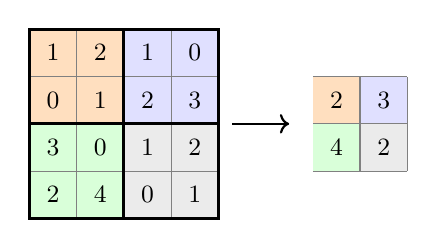
\begin{tikzpicture}
\def\c{0.6}
\fill[orange!25] (0,0) rectangle (2*\c,-2*\c);
\fill[blue!12] (2*\c,0) rectangle (4*\c,-2*\c);
\fill[green!15] (0,-2*\c) rectangle (2*\c,-4*\c);
\fill[black!8] (2*\c,-2*\c) rectangle (4*\c,-4*\c);
\draw[step=\c,black!50] (0,0) grid (4*\c,-4*\c);
\draw[very thick] (0,0) rectangle (4*\c,-4*\c);
\draw[very thick] (2*\c,0) -- (2*\c,-4*\c); \draw[very thick] (0,-2*\c) -- (4*\c,-2*\c);
\foreach \v [count=\i from 0] in {1,2,1,0,0,1,2,3,3,0,1,2,2,4,0,1} {
  \pgfmathtruncatemacro{\r}{\i/4}\pgfmathtruncatemacro{\q}{\i-4*\r}
  \node[font=\small] at ({(\q+0.5)*\c},{-(\r+0.5)*\c}) {\v};
}
\draw[->,thick] (4.3*\c,-2*\c) -- (5.5*\c,-2*\c);
\fill[orange!25] (6*\c,-1*\c) rectangle (7*\c,-2*\c);
\fill[blue!12] (7*\c,-1*\c) rectangle (8*\c,-2*\c);
\fill[green!15] (6*\c,-2*\c) rectangle (7*\c,-3*\c);
\fill[black!8] (7*\c,-2*\c) rectangle (8*\c,-3*\c);
\draw[step=\c,black!50,shift={(0,-1*\c)}] (6*\c,0) grid (8*\c,-2*\c);
\node[font=\small] at (6.5*\c,-1.5*\c) {2}; \node[font=\small] at (7.5*\c,-1.5*\c) {3};
\node[font=\small] at (6.5*\c,-2.5*\c) {4}; \node[font=\small] at (7.5*\c,-2.5*\c) {2};
\end{tikzpicture}
\end{adjustbox}
\end{column}
\end{columns}
\vskip1mm
\begin{itemize}
\item \code{nn.MaxPool2d(2)}: $2\times2$ 영역마다 \textbf{최댓값} 하나. 스트라이드를 따로 주지 않으면 창 크기와 같은 $2$
\item 학습할 매개변수가 \textbf{없다}. 채널마다 따로 계산하므로 채널 수는 그대로: $(N,30,24,24)\to(N,30,12,12)$
\end{itemize}
\end{frame}

\begin{frame}[fragile]{\code{nn.Flatten}: 완전연결 계층으로 넘기기}
\begin{lstlisting}
print(tuple(nn.Flatten()(torch.zeros(100, 30, 12, 12)).shape))
\end{lstlisting}
\begin{lstlisting}[style=outstyle]
(100, 4320)
\end{lstlisting}
\begin{itemize}
\item 첫 번째 차원(미니배치 $N$)은 \textbf{남기고} 나머지를 한 줄로: $30\times12\times12=4320$
\item \code{print(model)}에 나오는 \code{Flatten(start\_dim=1, end\_dim=-1)}: 1번 차원부터 끝까지 펼친다는 뜻
\item 그냥 \code{x.reshape(-1)}로 펼치면 미니배치까지 섞여 \code{(432000,)}이 되어 버린다
\item 이제 \code{nn.Linear(4320, 100)}에 넣을 수 있다
\end{itemize}
\vskip1mm
\begin{remarkbox}[세 계층의 대응]
\small
\centering
\begin{adjustbox}{max width=\linewidth}
\begin{tabular}{ll}
노트의 NumPy 구현 (\code{conv\_layers.py}) & PyTorch \\
\midrule
\code{Convolution(W, B, stride, pad)} & \code{nn.Conv2d(C, FN, kernel\_size, stride, padding)} \\
\code{Pooling(2, 2)} & \code{nn.MaxPool2d(2)} \\
\code{Flatten()} & \code{nn.Flatten()} \\
\end{tabular}
\end{adjustbox}
\end{remarkbox}
\end{frame}

% =================================================
\section{모델: \texttt{nn.Sequential}}
% =================================================

\begin{frame}[fragile]{모델 만들기}
\begin{lstlisting}
model = nn.Sequential(
    nn.Conv2d(1, 30, kernel_size=5),      # (N, 1, 28, 28) -> (N, 30, 24, 24)
    nn.ReLU(),
    nn.MaxPool2d(2),                      # -> (N, 30, 12, 12)
    nn.Flatten(),                         # -> (N, 4320)
    nn.Linear(30 * 12 * 12, 100),
    nn.ReLU(),
    nn.Linear(100, 10),
).to(device)
print(model)
print("number of parameters:", sum(p.numel() for p in model.parameters()))
\end{lstlisting}
\begin{itemize}
\item 계층 7개를 \textbf{순서대로} 나열했을 뿐이다. \code{class}를 따로 만들지 않았다
\item \code{nn.Linear(30 * 12 * 12, 100)}: 앞 계층의 출력 크기를 \textbf{직접 계산해서} 넣어야 한다
\begin{itemize}
\item 필터 크기나 패딩을 바꾸면 이 숫자도 바꿔야 한다. 틀리면 실행할 때 \code{shape} 오류가 난다
\end{itemize}
\item \code{.to(device)}: 모든 매개변수를 GPU로 (있으면)
\end{itemize}
\end{frame}

\begin{frame}[fragile]{\code{print(model)}의 출력}
\begin{lstlisting}[style=outstyle]
device: cuda
Sequential(
  (0): Conv2d(1, 30, kernel_size=(5, 5), stride=(1, 1))
  (1): ReLU()
  (2): MaxPool2d(kernel_size=2, stride=2, padding=0, dilation=1, ceil_mode=False)
  (3): Flatten(start_dim=1, end_dim=-1)
  (4): Linear(in_features=4320, out_features=100, bias=True)
  (5): ReLU()
  (6): Linear(in_features=100, out_features=10, bias=True)
)
number of parameters: 433890
\end{lstlisting}
\small
\begin{itemize}
\item 괄호 안의 번호 \code{(0)}--\code{(6)}: 계층의 순번. \code{model[0]}이 첫 번째 합성곱 계층 (뒤에서 필터를 꺼낼 때 쓴다)
\item \code{kernel\_size=(5, 5)}: 숫자 하나 \code{5}를 주면 가로세로 같은 크기로
\item \code{MaxPool2d}의 \code{stride=2}: 따로 주지 않아서 창 크기와 같아졌다
\item 이번 실행은 이 컴퓨터의 GPU(\code{cuda})에서 했다
\end{itemize}
\end{frame}

\begin{frame}[fragile]{계층마다 모양과 매개변수 수}
\begin{columns}[T,onlytextwidth]
\begin{column}{0.48\textwidth}
\begin{lstlisting}
h = torch.randn(100, 1, 28, 28)
for layer in model:
    h = layer(h)
    print(type(layer).__name__,
          tuple(h.shape))
\end{lstlisting}
\begin{lstlisting}[style=outstyle]
input      (100, 1, 28, 28)
Conv2d     (100, 30, 24, 24)
ReLU       (100, 30, 24, 24)
MaxPool2d  (100, 30, 12, 12)
Flatten    (100, 4320)
Linear     (100, 100)
ReLU       (100, 100)
Linear     (100, 10)
\end{lstlisting}
\end{column}
\begin{column}{0.48\textwidth}
\begin{lstlisting}
for name, p in model.named_parameters():
    print(name, tuple(p.shape), p.numel())
\end{lstlisting}
\begin{lstlisting}[style=outstyle]
0.weight  (30, 1, 5, 5)        750
0.bias    (30,)                 30
4.weight  (100, 4320)       432000
4.bias    (100,)               100
6.weight  (10, 100)           1000
6.bias    (10,)                 10
total parameters: 433890
\end{lstlisting}
\end{column}
\end{columns}
\vskip1mm
\small
\begin{itemize}
\item \code{for layer in model}: \code{Sequential}은 계층을 하나씩 꺼낼 수 있다 $\to$ 모양을 확인하는 좋은 방법 (\code{cnn\_torch\_demo.py})
\item 매개변수의 $99.6\%$가 \code{4.weight} (Flatten 다음의 Linear)에 있다. 합성곱 계층은 겨우 $780$개
\end{itemize}
\end{frame}

% =================================================
\section{학습과 평가}
% =================================================

\begin{frame}[shrink,fragile]{손실 함수, 최적화 기법, 학습, 평가}
\begin{columns}[T,onlytextwidth]
\begin{column}{0.50\textwidth}
\begin{lstlisting}[basicstyle=\codesmall]
loss_fn = nn.CrossEntropyLoss()
optimizer = torch.optim.Adam(model.parameters(), lr=0.001)

def train_one_epoch(model, loader):
    model.train()
    for xb, yb in loader:
        xb, yb = xb.to(device), yb.to(device)
        loss = loss_fn(model(xb), yb)
        optimizer.zero_grad()
        loss.backward()
        optimizer.step()
\end{lstlisting}
\end{column}
\begin{column}{0.47\textwidth}
\begin{lstlisting}[basicstyle=\codesmall]
@torch.no_grad()
def accuracy(model, loader):
    model.eval()
    correct, n = 0, 0
    for xb, yb in loader:
        xb, yb = xb.to(device), yb.to(device)
        correct += (model(xb).argmax(dim=1)
                    == yb).sum().item()
        n += len(yb)
    return correct / n
\end{lstlisting}
\end{column}
\end{columns}
\small
\begin{itemize}
\item \textbf{지난번 코드와 같다.} 모델이 CNN이 되었는데도 손실, 최적화, 학습, 평가 코드는 그대로
\item \code{loss.backward()}: 합성곱 계층의 역전파(노트에서 \code{col2im}까지 직접 짰던 것)도 autograd가 해 준다
\item \code{train\_one\_epoch}는 손실을 기록하지 않는다 (이번에는 검증 정확도만 본다)
\item 이 모델에는 Dropout, BatchNorm이 없어 \code{train()}/\code{eval()}이 결과를 바꾸지 않지만, 습관처럼 써 둔다
\end{itemize}
\end{frame}

\begin{frame}[fragile]{학습 반복과 실행 결과}
\begin{columns}[T,onlytextwidth]
\begin{column}{0.50\textwidth}
\begin{lstlisting}[basicstyle=\codesmall]
epochs = 10
val_acc = []
for epoch in range(1, epochs + 1):
    t0 = time.time()
    train_one_epoch(model, train_loader)
    val_acc.append(accuracy(model, val_loader))
    print(f"epoch {epoch:2d} | val acc "
          f"{val_acc[-1]:.4f} | "
          f"{time.time() - t0:.0f} s")
print(f"test acc "
      f"{accuracy(model, test_loader):.4f}")
\end{lstlisting}
\end{column}
\begin{column}{0.46\textwidth}
\begin{lstlisting}[style=outstyle,basicstyle=\codesmall]
epoch  1 | val acc 0.9754 | 4 s
epoch  2 | val acc 0.9840 | 3 s
epoch  3 | val acc 0.9826 | 3 s
epoch  4 | val acc 0.9868 | 4 s
epoch  5 | val acc 0.9860 | 3 s
epoch  6 | val acc 0.9860 | 3 s
epoch  7 | val acc 0.9880 | 3 s
epoch  8 | val acc 0.9850 | 3 s
epoch  9 | val acc 0.9888 | 3 s
epoch 10 | val acc 0.9894 | 3 s
test acc 0.9886
\end{lstlisting}
\end{column}
\end{columns}
\small
\begin{itemize}
\item \code{time.time()}: 지금 시각(초). epoch가 끝난 뒤 시각에서 빼면 걸린 시간
\item 첫 epoch에 검증 $97.5\%$, 10 epoch 뒤 test $98.86\%$
\item 이 코드는 마지막 epoch의 모델로 test를 한 번 본다 (가장 좋은 epoch를 저장하지 않는다)
\end{itemize}
\end{frame}

\begin{frame}{완전연결 신경망과 비교}
\centering
\small
\renewcommand{\arraystretch}{1.3}
\begin{tabular}{>{\raggedright}p{6.6cm}rcc}
\toprule
& \textbf{매개변수} & \textbf{epoch} & \textbf{test 정확도} \\
\midrule
\code{mnist\_torch.py} (학습 관련 기술)\\ 은닉층 4개 + BatchNorm, AdamW & $110610$ & 15 & $97.80\%$ \\
\code{mnist\_cnn\_torch.py}\\ 합성곱 1개 + 완전연결 2개, Adam & $433890$ & 10 & $98.86\%$ \\
\bottomrule
\end{tabular}
\raggedright
\vskip3mm
\begin{itemize}
\item 합성곱 계층 \textbf{하나}만 넣어도 test 오차가 $2.20\%$에서 $1.14\%$로 \textbf{절반 가까이} 준다
\item 매개변수가 많아서가 아니다: 합성곱 계층의 매개변수는 $780$개뿐이다
\item 합성곱은 이미지의 \textbf{공간 구조}(이웃한 픽셀)를 쓴다. 펼쳐 넣는 완전연결 신경망은 이 정보를 버린다
\end{itemize}
\end{frame}

\begin{frame}{GPU와 CPU, 그리고 실행할 때마다 다른 결과}
\centering
\small
\renewcommand{\arraystretch}{1.3}
\begin{tabular}{lccc}
\toprule
\textbf{같은 코드, 이 컴퓨터에서} & \textbf{epoch당 시간} & \textbf{10 epoch 검증} & \textbf{test} \\
\midrule
GPU (RTX 3050), 1회째 & 약 $3$초 & $98.94\%$ & $98.86\%$ \\
GPU (RTX 3050), 2회째 & 약 $3$초 & $98.76\%$ & $98.61\%$ \\
CPU & 약 $10$초 & $98.96\%$ & $98.76\%$ \\
\bottomrule
\end{tabular}
\raggedright
\vskip3mm
\begin{itemize}
\item GPU가 CPU보다 약 $3$배 빠르다. 코드는 \textbf{한 글자도} 바꾸지 않았다 (\code{device}만 달라짐)
\item \code{torch.manual\_seed(0)}을 고정했는데도 GPU에서 두 번 돌린 결과가 \textbf{다르다}
\begin{itemize}
\item GPU는 수많은 덧셈을 동시에 하므로 더하는 \textbf{순서}가 실행마다 달라질 수 있고, 부동소수점에서는 순서가 바뀌면 마지막 자리가 달라진다
\item 작은 차이가 학습을 거치며 쌓인다. 정확도 $0.2$--$0.3\%$p 정도의 차이는 \textbf{우연}의 범위이다
\end{itemize}
\item 그래서 설정을 비교할 때는 여러 번 실행해 평균을 보는 것이 안전하다
\end{itemize}
\end{frame}

% =================================================
\section{학습한 필터 보기}
% =================================================

\begin{frame}[fragile]{첫 번째 합성곱 계층의 필터 꺼내기}
\begin{lstlisting}
# the 30 filters of the first layer: model[0].weight has shape (30, 1, 5, 5)
filters = model[0].weight.detach().cpu().numpy()
fig, axes = plt.subplots(1, 30, figsize=(12, 0.9))
for k, ax in enumerate(axes):
    ax.imshow(filters[k, 0], cmap="gray", interpolation="nearest")
    ax.set_xticks([])
    ax.set_yticks([])
fig.savefig(os.path.join(FIG_DIR, "cnn_torch_filters.png"), dpi=200, bbox_inches="tight")
plt.close(fig)
\end{lstlisting}
\small
\begin{itemize}
\item \code{model[0]}: \code{Sequential}의 0번 계층 $=$ \code{Conv2d}. \code{.weight}: $(30,1,5,5)$
\item \code{.detach()}: 기울기 추적을 끊고 $\to$ \code{.cpu()}: GPU에서 가져오고 $\to$ \code{.numpy()}: NumPy 배열로. matplotlib은 NumPy 배열을 그린다
\item \code{filters[k, 0]}: $k$번째 필터의 $0$번 채널 $\to$ $5\times5$ 배열 하나
\item \code{plt.subplots(1, 30)}: 한 줄에 칸 30개. \code{interpolation="nearest"}: 픽셀을 흐리게 보간하지 않고 네모 그대로
\end{itemize}
\end{frame}

\begin{frame}{학습한 필터: \code{cnn\_torch\_filters.png}}
\centering

\includegraphics[width=\linewidth]{cnn_torch_filters.png}
\figcap{GPU 1회째 실행에서 학습한 첫 번째 합성곱 계층의 필터 $30$개 (밝을수록 큰 값)}
\vskip3mm
\raggedright
\begin{itemize}
\item 밝은 부분과 어두운 부분이 나뉜 필터들: 여러 방향의 \textbf{에지}(밝기가 바뀌는 곳)에 반응한다
\item 처음에는 무작위였던 숫자들이 학습을 거쳐 이런 모양이 되었다 (\code{nn.Conv2d}의 기본 초기화는 균등분포)
\item 실행할 때마다 필터의 순서와 모양은 달라진다. 비슷한 \textbf{종류}의 필터가 나오는 것이 중요하다
\end{itemize}
\end{frame}

% =================================================
\section{정리와 실습}
% =================================================

\begin{frame}{정리}
\begin{keybox}[이번 시간의 핵심]
\small
\begin{itemize}\setlength{\itemsep}{0.6mm}
\item 이미지 미니배치는 $(N,C,H,W)$ 텐서: \code{reshape(-1, 1, 28, 28)}
\item \code{nn.Conv2d(C, FN, kernel\_size, stride, padding)}: 가중치 $(FN,C,FH,FW)$, 편향 $(FN,)$.
출력 크기 $\frac{H+2P-FH}{S}+1$
\item \code{nn.MaxPool2d(2)}: $2\times2$마다 최댓값, 매개변수 없음. \code{nn.Flatten()}: 미니배치 차원은 남기고 펼침
\item 모델은 \code{nn.Sequential}로 나열. \code{Linear}의 입력 크기($30\cdot12\cdot12$)는 직접 계산
\item 손실, 최적화, 학습 루프, 평가는 완전연결 신경망과 \textbf{같다}
\item 합성곱 계층 하나로 test 정확도 $97.8\%\to98.9\%$. 같은 코드가 GPU에서 약 $3$배 빠르다
\item GPU 결과는 실행마다 조금 다르다: 작은 차이는 우연의 범위
\end{itemize}
\end{keybox}
\end{frame}

\begin{frame}{실습 문제}
\small
\begin{enumerate}
\item \code{nn.Conv2d(1, 30, kernel\_size=5, padding=2)}로 바꾸면 \code{Linear}의 입력 크기는 얼마로 바꿔야 하는가? 먼저 계산하고 실행해 보자
\item 필터 수를 $30$에서 $10$, $60$으로 바꿔 매개변수 수와 test 정확도를 비교하기
\item 합성곱 $\to$ ReLU $\to$ 풀링을 \textbf{한 번 더} 쌓기 (\code{nn.Conv2d(30, 60, kernel\_size=3)}). 각 계층의 모양을 \code{for layer in model}로 확인하기
\item LeNet과 비슷한 신경망 만들기: \code{Conv2d(1, 6, 5, padding=2)} $\to$ \code{ReLU} $\to$ \code{MaxPool2d(2)} $\to$ \code{Conv2d(6, 16, 5)} $\to$ \code{ReLU} $\to$ \code{MaxPool2d(2)} $\to$ \code{Flatten} $\to$ \code{Linear(?, 120)} $\to$ \code{Linear(120, 84)} $\to$ \code{Linear(84, 10)}
\item 합성곱 뒤에 \code{nn.BatchNorm2d(30)}을 넣어 보기. 이번에는 \code{model.train()}/\code{model.eval()}이 결과를 바꾼다
\item 학습 뒤 test 이미지 한 장을 \code{model[:3]}에 넣어 특징 맵 30장 \code{(1, 30, 12, 12)}을 그리기 (힌트: \code{Sequential}도 잘라 쓸 수 있다)
\item 가장 좋은 epoch의 모델을 \code{copy.deepcopy(model.state\_dict())}로 저장하도록 고치기
\end{enumerate}
\end{frame}

\end{document}
